\newpage
\section{Diagnostic Tools for the nlme package}


With the nlme package, the generic function \texttt{lme()} fits a linear mixed-effects model in the formulation described in Laird and Ware (1982) but allowing for nested random effects. 

The within-group errors are allowed to be correlated and/or have unequal variances, which is very important in fitting the models for Roy's Tests

The nlme package has a limited set of diagnostic tools that can be used to assess the model fit. A review of the package manual is sufficient to get a sense of the package's capability in that regard.


\newpage


\subsection{Conditional and Marginal Residuals}
A residual is the difference between an observed quantity and its estimated or predicted value. For LME models, \citet{schab} describes two types of residuals, marginal residuals and conditional residuals. 

\begin{itemize}
	\item A marginal residual is the difference between the observed data and the estimated (marginal) mean, $r_{mi} = y_i - x_0^{\prime} \hat{b}$
	\item A conditional residual is the difference between the observed data and the predicted value of the observation,
	$r_{ci} = y_i - x_i^{\prime} \hat{b} - z_i^{\prime} \hat{\gamma}$	
\end{itemize} 
In a model without random effects, both sets of
residuals coincide \citep{schab} . We shall revert to this matter in due course.



%\subsection{Marginal and Conditional Residuals}




In linear mixed effects models, diagnostic techniques may consider `conditional' residuals. A conditional residual is the difference between an observed value $y_{i}$ and the conditional predicted value $\hat{y}_{i} $.

\[ \hat{\epsilon}_{i} = y_{i} - \hat{y}_{i} = y_{i} - ( X_{i}\hat{\beta} + Z_{i}\hat{b}_{i}) \]

However, using conditional residuals for diagnostics presents difficulties, as they tend to be correlated and their variances may be different for different subgroups, which can lead to erroneous conclusions.

%========================================================%

\newpage
\subsection{Residual Analysis for MCS}

\begin{figure}[h!]
	\centering
	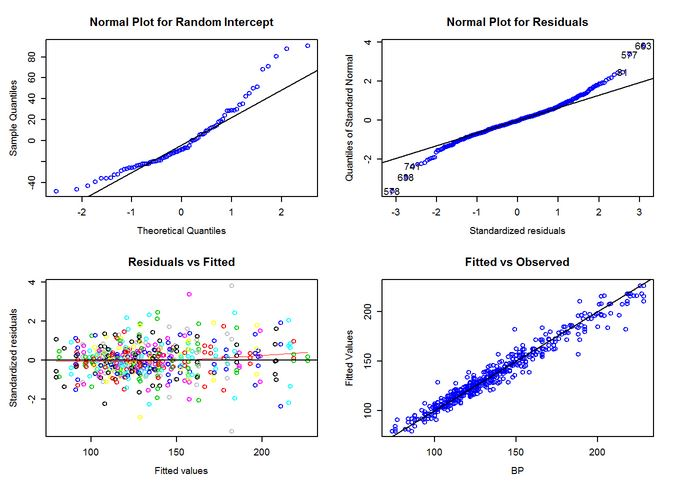
\includegraphics[width=0.9\linewidth]{images/ResidPlot}
	\caption{}
	\label{fig:ResidPlot}
\end{figure}


\subsection{PRESS Residuals and PRESS Statistic}
% % - Wikipedia
In statistics, the predicted residual sum of squares (PRESS) statistic is a form of cross-validation used in regression analysis to provide a summary measure of the fit of a model to a sample of observations that were not themselves used to estimate the model. It is calculated as the sums of squares of the prediction residuals for those observations.

A fitted model having been produced, each observation in turn is removed and the model is refitted using the remaining observations. The out-of-sample predicted value is calculated for the omitted observation in each case, and the PRESS statistic is calculated as the sum of the squares of all the resulting prediction errors:[4]
\[\mbox{PRESS} =\sum_{i=1}^n (y_i - \hat{y}_{i, -i})^2 \]
Given this procedure, the PRESS statistic can be calculated for a number of candidate model structures for the same dataset, with the lowest values of PRESS indicating the best structures. Models that are over-parameterised (over-fitted) would tend to give small residuals for observations included in the model-fitting but large residuals for observations that are excluded.

% % - http://support.sas.com/documentation/cdl/en/statug/63347/HTML/default/viewer.htm#statug_mixed_sect027.htm
An (unconditional) predicted value is $\hat{y}_i = x^{\prime}_i \boldsymbol{\hat{\beta}}$, where 
the vector $x_i$ is the $i$th row of $\boldsymbol{X}$. For an \texttt{lme} object, such as our fitted model \texttt{JS.roy1}, the predicted values for each subject can be determined using the \texttt{coef.lme} function.
\begin{framed}
	\begin{verbatim}
	> JS.roy1 %>% coef %>% head(5)
	methodJ   methodS
	74     84.31724  91.08404
	36     91.54994  97.05548
	3      81.16581  96.48653
	62     92.09493  90.89073
	31     88.41411 103.38802
	\end{verbatim}
\end{framed}



The (raw) residual is given as $\varepsilon_i = y_i - \hat{y}_i$. The PRESS residual is
similarly constructed, using the predicted value for observation $i$ with a model fitted from reduced data.
\[ \varepsilon_{i(U)} = y_i - x^{\prime}_i \boldsymbol{\hat{\beta}}_{(U)} \]
The PRESS statistic is the sum of the squared PRESS residuals:
\[ PRESS = \sum \varepsilon^2_{i(U)} \]
where the sum is over the observations in $\boldsymbol{U}$.


%---------------------------------------------------------------------------%
\newpage

Pinheiro and Bates provide some insight into how to compute and interpret model diagnostic plots for lme models. Unfortunately this aspect of LME theory is not as expansive as the corresponding body of work for Linear Models.
\section{Checking the Assumption by Method}


\subsection{Residual Analysis}


\textbf{qqnorm.lme}
% {nlme}	R Documentation
Normal Plot of Residuals or Random Effects from an lme Object

Description

Diagnostic plots for assessing the normality of residuals and random effects in the linear mixed-effects fit are obtained. 
The form argument gives considerable flexibility in the type of plot specification. 
A conditioning expression (on the right side of a | operator) always implies that different panels are used 
for each level of the conditioning factor, according to a Trellis display.

%============================================================================== %

%====================================================================%
\subsubsection{Residuals plots}

lme allows to plot the residuals in the following ways:

\begin{framed}
	\begin{verbatim}
	res_lme=residuals(model_lme)
	plot(res_lme)
	qqnorm(res_lme)
	qqline(res_lme)
	plot(model_lme)
	\end{verbatim}
\end{framed}

%==============================================================%


\subsection{Diagnostic Plots for LME models}



When the \texttt{plot} function calls the model object, the residual plot is produced.





\begin{framed}
	\begin{verbatim}
	plot(JS.roy1, which=c(1) )
	\end{verbatim}
\end{framed}


\begin{figure}[h!]
	\centering
	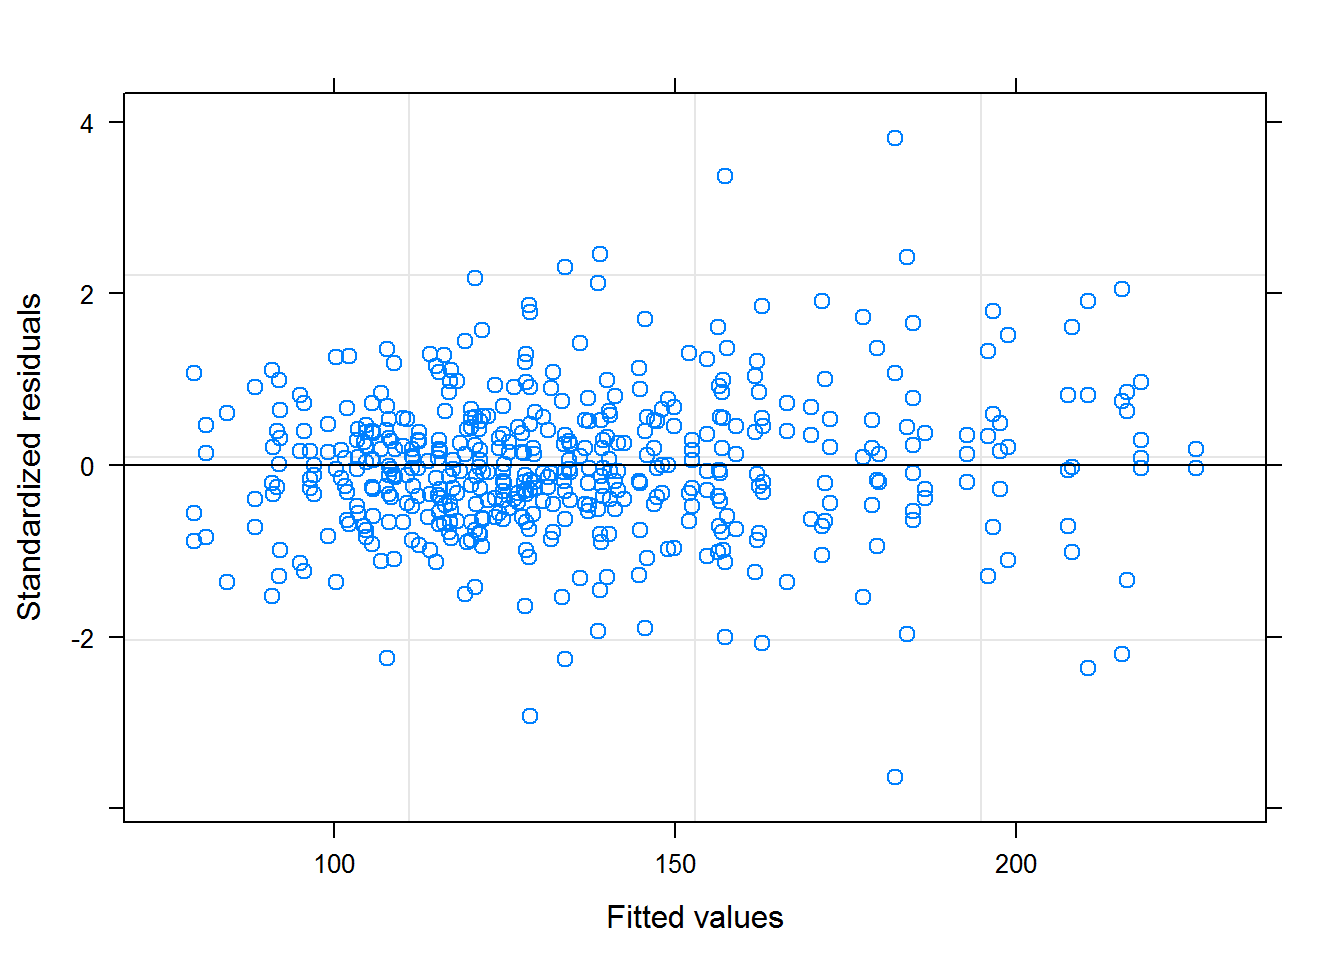
\includegraphics[width=0.9\linewidth]{images/ResidPlot1}
	\caption{}
	\label{fig:ResidPlot1}
\end{figure}
LME models assume that the residuals of the model are normally distributed. A Normal probability plot can be constructed to check this assumption. Commonly used \texttt{R} commands can be used to construct the plot.
\newpage

\begin{framed}
	\begin{verbatim}
	qqnorm(resid(JS.roy1),pch="*",col="red")
	qqline(resid(JS.roy1),col="blue")
	\end{verbatim}
\end{framed}




\begin{figure}[h!]
	\centering
	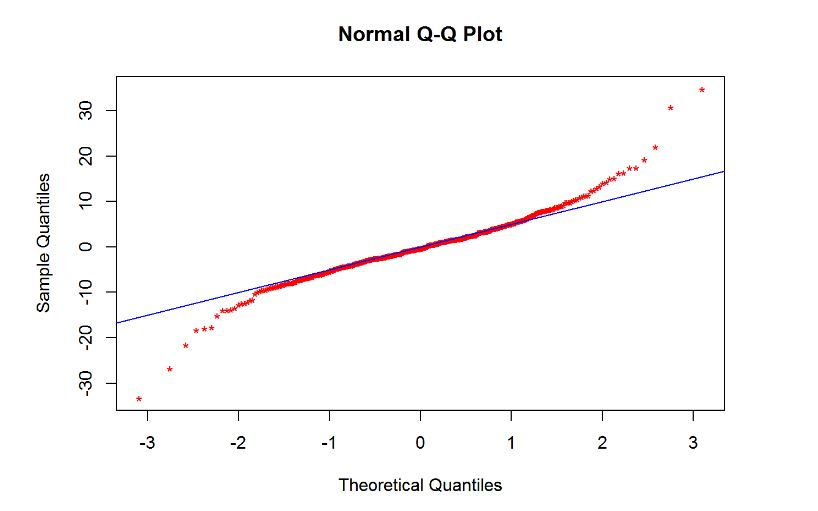
\includegraphics[width=0.7\linewidth]{images/Resid-newplot}
	\caption{}
	\label{fig:Resid-newplot}
\end{figure}

\begin{framed}
	\begin{verbatim}
	table(dat$method[1:255])
	## 
	##   J   S 
	## 255   0
	table(dat$method[256:510])
	## 
	##   J   S 
	##   0 255
	\end{verbatim}	
\end{framed}
%==================================================================================%
\newpage
\begin{framed}
\begin{verbatim}
plot(roy.NLME, resid(., type = "p") ~ fitted(.) | method, 
   abline = 0, id=.05)
\end{verbatim}
\end{framed}
\begin{figure}
\centering
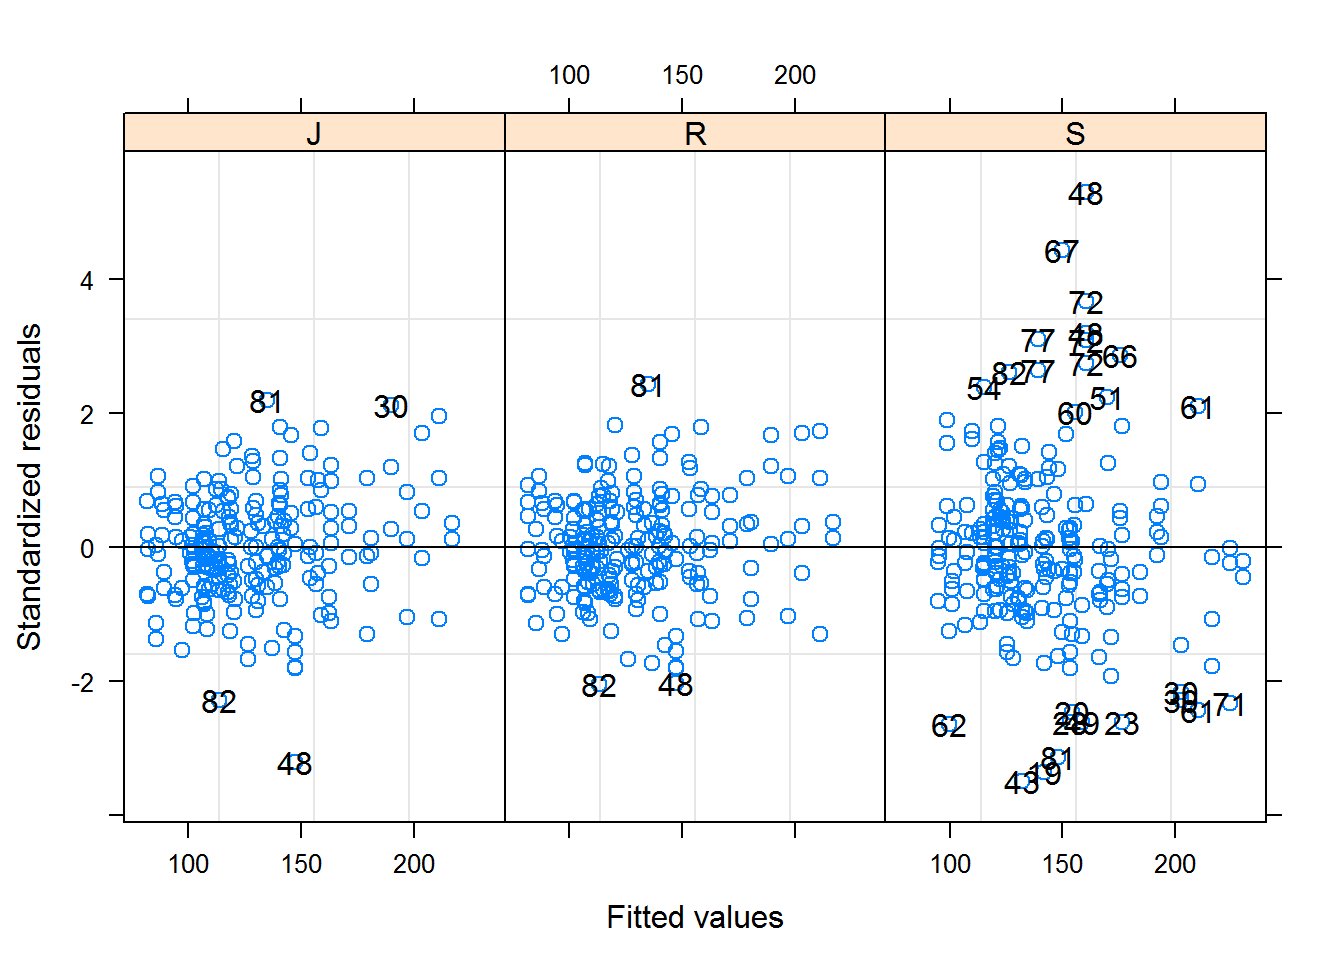
\includegraphics[width=0.9\linewidth]{images/bloodnlmeResidPlot2}
\caption{}
\label{fig:blood}
\end{figure}


\subsubsection{Cooks distance- Predict means thing here}
Cook's Distance is a model diagnostic measure of an observation that is a measure of aggregate impact of each observation on the group of regression coefficients. Observations, or sets of observations, that have high Cook's distance usually have high resdiauls. We will revisit Cook's distance fully in due cource.

Cook's Distance is a good measure of the influence of an observation that is a measure of aggregate impact of each observation on the group of regression coefficients, as well as the group of fitted values.

The \texttt{CookD} fucntion , from the predictmeans R package, produces Cook’s distance plots for an LME model 
 (predictmeans)



\begin{framed}
\begin{verbatim}
library(predictMeans)
CookD(model, group=method, plot=TRUE, idn=5, newwd=FALSE)
\end{verbatim}
\end{framed}


\begin{verbatim}
## Cook's Distance

\end{verbatim}

The particular cases that we will omit for the subsequent analysis are subjects 68,78 and 80.

\subsubsection{Reduced Data Set}
It is important to determine if a specific group of cases or subjects give rise to the lack of agreement in the methods. If one were to examine fitted model if these cases were removed.

\begin{framed}
\begin{verbatim}

blood.red <- blood[!(blood$subject %in% c(68,78,80)),]
dim(blood.red)
# 27 observations should be removed.

blood.NLME.red <-lme(BP ~ method-1 , random=~1|subject,data = blood.red)
plot(blood.NLME.red, resid(., type = "p") ~ fitted(.) | method, abline = 0, id=.05)
\end{verbatim}
\end{framed}

In this instance, we conclude that there is a systemic diagreement between method S and the other two methods, and that lack of agreement can not be sourced to a handful of cases.
\begin{figure}[h!]
	\centering
	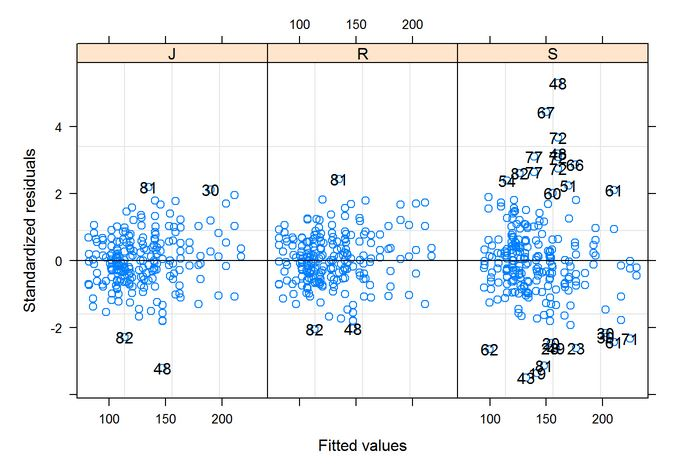
\includegraphics[width=0.7\linewidth]{images/bloodnlmeResidPlot2B}
\end{figure}


\newpage


\chapter{Using DFBETAs from LME Models to Assess Agreement}
	
	
	\citet{schab} examines the use and implementation of influence measures in LME models.
	
	Influence is understood to be the ability of a single or multiple data points, through their presences or absence in the data, to alter important aspects of the analysis, yield qualitatively 	different inferences, or violate assumptions of the statistical
	model \citep{schab}.
	
	Outliers are the most noteworthy data points in an analysis, and an objective of influence analysis is how influential they are,
	and the manner in which they are influential.
	
	\citet{schab} describes a simple procedure for quantifying influence.
	\begin{itemize}
		\item Firstly a model should be fitted to the data, and
		estimates of the parameters should be obtained.
		\item The second step is that either single or multiple data points, specifically outliers,
		should be omitted from the analysis, with the original parameter
		estimates being updated.
		\item  The final step of the procedure is comparing the 	sets of estimates computed from the entire and reduced data sets
		to determine whether the absence of observations changed the
		analysis.
	\end{itemize}
	   This is known as `\textit{leave one out} or \texttt{leave k
	out' analysis}.
	


	
	
	\subsection{Influence}
	
	Influence arises at two stages of the LME model. Firstly when $\mathbf{V}$ is estimated by $\hat{V}$, and subsequent
	estimations of the fixed and random regression coefficients $\mathbf{\beta}$ and $u$, given $\mathbf{\hat{V}}$.
	
	%- The Mahalanobis distance is a measure of the distance between a point P and a distribution D, introduced by P. C. Mahalanobis in 1936.
	4 It is a multi-dimensional generalization of the idea of measuring how many standard deviations away P is from the mean of D. 
	
	This distance is zero if P is at the mean of D, and grows as P moves away from the mean: Along each principal component axis, it measures the 
	number of standard deviations from P to the mean of D. If each of these axes is rescaled to have unit variance, then Mahalanobis distance corresponds to standard Euclidean distance in the transformed space. Mahalanobis distance is thus unitless and scale-invariant, and takes into account the correlations of the data set.

	%============================================================================%
	\subsection*{Influence() - Description}
	\texttt{influence()} is the workhorse function of the \texttt{influence.ME} package. 
	
	
	Based on a priorly estimated mixed effects regression model (estimated using lme4), the \texttt{influence()} function iteratively 
	
	modifies the mixed effects model to neutralize the effect a grouped set of data has on the parameters, and which 
	
	returns returns the fixed parameters of these iteratively modified models. 
	
	These are used to compute measures of influential data.
	
	
	
	
	\subsection*{Usage}
	\begin{framed}
		\begin{verbatim}
		
		influence(model, group=NULL, select=NULL, obs=FALSE, 
		gf="single", count = FALSE, delete=TRUE, ...)
		\
		\end{verbatim}
	\end{framed}
	
	
	The \texttt{influence()} function was known as the \texttt{estex()} command in previous versions of the influence.ME pacakge
	%===========================================================================%
	%- http://support.sas.com/documentation/cdl/en/statug/63347/HTML/default/statug_reg_sect040.htm

	
	
	
	
	


	\subsection{PRESS} %1.16.2
	The prediction residual sum of squares (PRESS) is an value associated with this calculation. When fitting linear models, PRESS can be used as a criterion for model selection, with smaller values indicating better model fits.
	\begin{equation}
	PRESS = \sum(y-y^{(k)})^2
	\end{equation}
	
	
	\begin{itemize}
		\item $e_{-Q} = y_{Q} - x_{Q}\hat{\beta}^{-Q}$
		\item $PRESS_{(U)} = y_{i} - x\hat{\beta}_{(U)}$
	\end{itemize}
	



%============================================================================= %
\section{Application of DFBETAs in MCS Analysis}


When in an MCS study. DFBetas can be used as a proxy measurement, allowing simple techniques to be used for assessing agreement.



\chapter{Model Diagnostics for MCS}

%-------------------------------------------------------------------------%
\begin{abstract}
Model diagnostic techniques, well established for classical models, have since been adapted for use with linear mixed effects models. However, diagnostic techniques for LME models are inevitably more difficult to implement, due to the increased complexity. \\ \bigskip


\citet{schab} describes the examination of model-data agreement as comprising several elements; \begin{itemize}
		\item residual analysis, 
		\item goodness of fit, 
		\item collinearity diagnostics
		\item influence analysis.
	\end{itemize} 
	
This chapter is comprised of two sections:
\begin{enumerate}
	\item Residual Diagnostics
	\item Influence Diagnostics
\end{enumerate}
\end{abstract}

%=============================================================================== %
\newpage
\section{Introduction}
In statistical modelling, the process of model validation is a critical step, but also a step that is too often overlooked. A very simple procedure is to examine well known
metrics, such as the AIC and $R^2$ measures. However, using a small handful of simple measures and methods is insufficient to properly assess the quality of a fitted model. To do so properly, a full and comprehensive
analysis that tests of all of the assumptions, as far as possible, must be carried out. 

A statistical model, whether of the fixed-effects or mixed-effects variety, represents how you think your data were generated. Following model specification and estimation, it is of interest to explore the model-data
agreement by raising pertinent questions. Further to the analysis of residuals, \citet{schab} recommends the examination of the following questions.
\begin{itemize}
	\item Does the model-data agreement support the model assumptions?
	\item Should model components be refined, and if so, which components? For example, should certain explanatory variables
	be added or removed, and is the covariance of the observations properly specified?
	\item Are the results sensitive to model and/or data? Are individual data points or groups of cases particularly
	influential on the analysis?
\end{itemize}
\newpage





\newpage
\subsection{Cook's Distance}
\citet{CPJ} develops \index{case deletion diagnostics} case deletion diagnostics, in particular the equivalent of \index{Cook's distance} Cook's distance, a well-known metric, for diagnosing influential observations when estimating the fixed effect parameters and variance components. Deletion diagnostics provide a means of assessing the influence of an observation (or groups of observations) on inference on the estimated parameters of LME models. 
%We shall provide a fuller discussion of Cook's distance in due course.
Cook's Distance is a good measure of the influence of an observation that is a measure of aggregate impact of each observation on the group of regression coefficients, as well as the group of fitted values.
%Cook's Distance is proportional to the sum of the squared differences between predictions made with all observations in the analysis and predictions made leaving out the observation in question. 
If the predictions are the same with or without the observation in question, then the observation has no influence on the regression model. If the predictions differ greatly when the observation is not included in the analysis, then the observation is influential.

%======================================================================================= %
\newpage
% Hence the name deletion diagnostics and case-deletion diagnostics. 
\subsubsection{Cook's Distance for Blood Data}
\begin{figure}[h!]
	\centering
	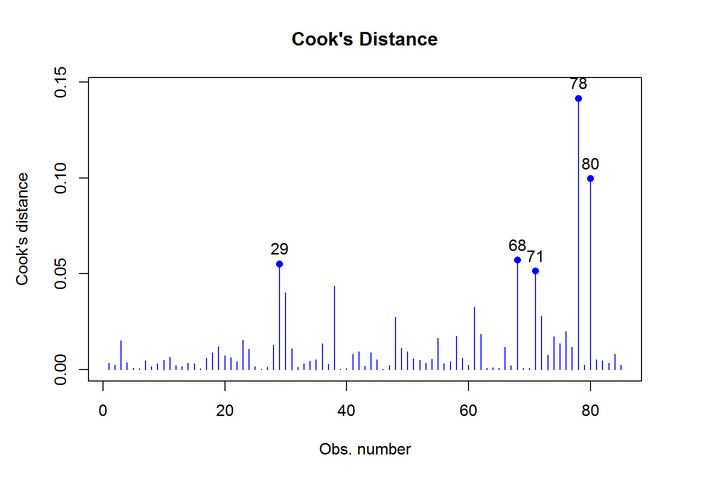
\includegraphics[width=0.9\linewidth]{images/CooksDistancePlot-JS-Roy}
%	\caption{}
%	\label{fig:CooksDistancePlot-JS-Roy}
\end{figure}


\newpage
\subsection{Deviance}
In statistics, deviance is a quality of fit statistic for a model that is often used for statistical hypothesis testing. It is a generalization of the idea of using the sum of squares of residuals in ordinary least squares to cases where model-fitting is achieved by maximum likelihood.

%-----------------------------------%


\bibliography{DB-txfrbib}
\end{document}
%================================================================================ %
